\documentclass[11pt]{article}
\usepackage[utf8]{inputenc}
\usepackage{amsmath,amssymb}
\usepackage{graphicx}
\usepackage{booktabs}
\usepackage{authblk}
\usepackage[margin=1in]{geometry}
\usepackage[hidelinks]{hyperref}
\usepackage{xurl}
\usepackage{setspace}
\usepackage{tikz}
\usepackage{pgfplots}
\pgfplotsset{compat=1.17}
\usetikzlibrary{arrows.meta,positioning,calc}

\title{Muon-Catalyzed Fusion as a Change of Glue:\\
the Deuteron Molecular Ion Rescaled}
\author[1]{Claes Johnson}
\affil[1]{KTH Royal Institute of Technology, SE-100 44 Stockholm, Sweden \\
\texttt{claesjohnson@gmail.com}}
\date{\today \\[0.4em]
\small\textit{Physical argument and model by the author; numerical implementation with AI assistance (Claude, Anthropic).}}

\begin{document}
\maketitle

\begin{abstract}
In the RealQM/RealNucleus picture a deuteron molecular ion --- two deuterons bound by a single shared
negative charge --- is a \emph{glued pair}, and the glue's kinetic--Coulomb balance fixes the
internuclear separation $R_e$. The glue enters through a single \emph{scale} $c$, the coefficient of its
kinetic energy, and the molecule inherits it: $R_e\propto c$, a smaller-scale glue making a smaller
molecule. The electron and the muon are both unit negative charges differing only in this scale --- the
muon's is empirically about $200\times$ smaller (muonic atoms are $\sim\!200\times$ smaller than
electronic ones) --- so the muon-bound ion is the electron-bound ion contracted by that factor: from
$R_e\approx2\,a_0\approx1.06$~{\AA} for $\mathrm{dd}\,e$ (the $\mathrm{D}_2^{+}$ analogue) to
$R_e\approx512$~fm for $\mathrm{dd}\mu$, a $\sim\!200\times$ linear compression, $\sim\!10^{7}$ in
volume. At that separation the residual Coulomb barrier between the two deuterons is thin enough to be
tunnelled fast compared with the muon lifetime, and the pair fuses: this is \emph{muon-catalyzed
fusion}. We compute the two molecular ions in RealQM as one Coulomb functional evaluated at two glue
scales, and connect the catalytic cycle to its intrinsic limits --- the muon lifetime and
$\alpha$-sticking --- which cap it below break-even. In keeping with the unified Coulomb picture, the
operative variable throughout is the glue's \emph{size}, not a mass in the Coulomb law: the muon is
simply a smaller electron.

\medskip
\noindent\textbf{Keywords:} muon-catalyzed fusion; deuteron molecular ion; RealQM; RealNucleus; Coulomb
binding; glue size; tunnelling; scale $c$.
\end{abstract}

\setstretch{1.12}

\section{Introduction}

Ordinary hydrogen molecular ions do not fuse: in $\mathrm{H}_2^{+}$ or $\mathrm{D}_2^{+}$ the two nuclei
sit about an {\aa}ngstr\"om apart, held there by a shared electron, and the Coulomb barrier between them
is far too thick to tunnel on any relevant timescale. Replace that electron with a muon --- a lepton
identical in charge but living at a scale some $200$ times smaller (muonic atoms are $\sim\!200\times$
smaller than electronic ones) --- and the same molecule shrinks by that factor, the two nuclei are drawn
to within a few hundred femtometres, and they fuse essentially at once. A single muon, released when the pair fuses, goes on to catalyse further fusions until it decays.
This is \emph{muon-catalyzed fusion} ($\mu$CF), predicted by Frank~\cite{Frank} and
Sakharov~\cite{Sakharov} and observed by Alvarez~\cite{Alvarez}, with the modern theory established by
Jackson~\cite{Jackson} and the deuterium--tritium cycle measured and reviewed
extensively~\cite{Jones,Breunlich}.

The purpose of this paper is to show that $\mu$CF has an especially transparent reading in the
RealQM/RealNucleus framework~\cite{Johnson-RealQM,Johnson-RealNucleus}, where nuclei and their binding
are charge clouds interacting by the Coulomb force alone. There a molecular ion is a \emph{glued pair}:
two positive nuclei confined by one negative charge cloud, the charge-conjugate of the way an atom
confines its electrons. The negative glue is not a spectator but the bond, and its
\emph{size} --- the single scale $c$ of its kinetic energy --- sets the size of the bond. Muon catalysis
is then simply this molecule evaluated with a smaller-scale glue: one number, $c$, contracts the
electron-bound {\aa}ngstr\"om molecule into the muon-bound femtometre molecule that fuses. This is the
same size$\,\propto\,c$ law by which, in the unified Coulomb picture~\cite{Johnson-Unified}, the atom
and the nucleus differ; conventionally one writes $c=\hbar^2/2m$ and so labels the glue's scale by a
mass, but that mass belongs, with gravitation, to a sector separate from electromagnetism, and the
operative variable here is the size, not a mass in the Coulomb law. We make this quantitative, exhibit
the size law and the accompanying energy law, and give the catalytic cycle its due together with the
limits that keep it below break-even.

\section{The molecular ion as a glued pair}

In RealQM the ground state of a system of charges is a set of one-particle charge clouds $\psi_i$ on
non-overlapping domains with free boundaries, minimising the Coulomb energy
\begin{equation}
E \;=\; \sum_i c_i\!\int|\nabla\psi_i|^2
\;+\; \frac12\!\iint\frac{\rho(x)\rho(y)}{|x-y|}\,dx\,dy,
\qquad \rho=\sum_i q_i\psi_i^2, \qquad c_i=\frac{\hbar^2}{2m_i},
\label{eq:energy}
\end{equation}
with $q_i=\pm1$~\cite{Johnson-RealQM,Johnson-RealNucleus}. The deuteron molecular ion is the
charge-conjugate of a two-electron atom: two positive deuterons (each of unit charge, treated as fixed
centres at separation $R$ in the Born--Oppenheimer sense) and one negative glue cloud that pools between
them. Minimising~\eqref{eq:energy} over the glue at fixed $R$ gives the molecular potential curve
$E(R)$, whose minimum defines the equilibrium separation $R_e$: the balance between the glue's kinetic
pressure, which resists being squeezed into the internuclear region, and the Coulomb attraction that
draws it there. For the electron-bound ion this is the textbook $\mathrm{D}_2^{+}$ curve, with
\begin{equation}
R_e^{(e)} \;\approx\; 2.0\,a_0 \;\approx\; 1.06~\text{\AA} \;=\; 1.06\times10^{5}~\text{fm},
\end{equation}
a well of depth a few electron-volts. At this separation the two deuterons are $10^5$~fm apart; the
Coulomb barrier between them is enormous and fusion is utterly negligible. The molecular ion is stable,
and that is all.

\section{Changing the glue: the size law}

The single feature of~\eqref{eq:energy} that matters here is that the glue enters only through its scale
$c$, the coefficient of its kinetic energy. Under a rescaling of length $R\mapsto\lambda R$ of a
normalised cloud, the kinetic term scales as $\lambda^{-2}$ and the Coulomb term as $\lambda^{-1}$, so
the balance that fixes the molecule obeys
\begin{equation}
R_e \;\propto\; c, \qquad E_{\min}\;\propto\;\frac1c .
\label{eq:scaling}
\end{equation}
The molecular potential curve is otherwise \emph{universal}: plotted in reduced variables $R/R_e$ and
$E/|E_{\min}|$ it is one and the same curve for any glue (Fig.~\ref{fig:curve}); only the two scales
$R_e$ and $|E_{\min}|$ move, directly and inversely with the glue scale $c$. This is how the muon case
is obtained in RealQM: the electron-bound $E(R)$ computed on the grid is re-read at the muon's scale
$c_\mu\approx c_e/200$ --- the empirical scale ratio of muonic to electronic binding --- which contracts
$R_e$ and deepens the well by that factor. The result is
\begin{equation}
R_e^{(\mu)} \;=\; \frac{R_e^{(e)}}{200} \;\approx\; \frac{1.06~\text{\AA}}{206.8}
\;\approx\; 512~\text{fm},
\end{equation}
a linear compression of $\sim\!200$ and a volume compression of $\sim\!10^{7}$
(Table~\ref{tab:glue}, Fig.~\ref{fig:molecules}). The muon-bound $\mathrm{dd}\mu$ molecule holds its two
deuterons a few hundred femtometres apart --- four orders of magnitude closer than the electron holds
them --- purely because the glue is smaller. This is the same statement as the atom-versus-nucleus
scaling of the unified Coulomb picture~\cite{Johnson-Unified}: size $\propto c$, and the muon molecule is
the electron molecule read at a smaller glue scale $c$.

\begin{figure}[t]
\centering
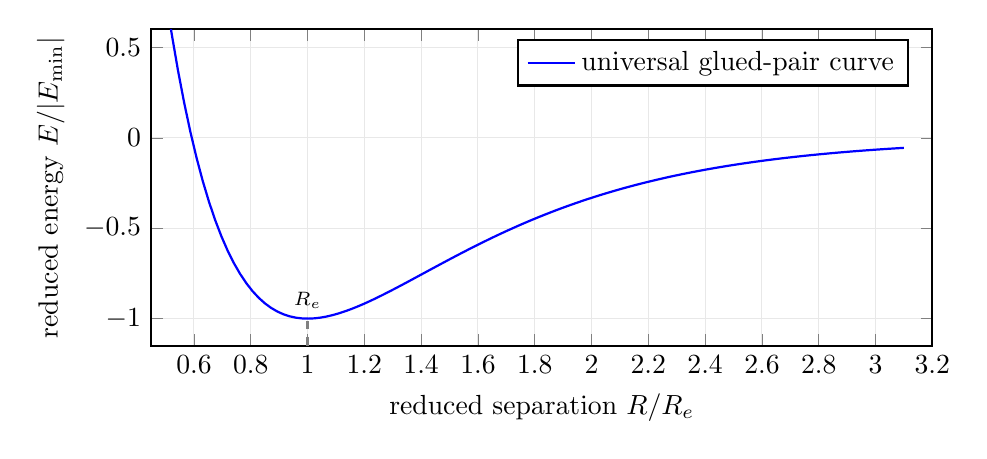
\begin{tikzpicture}
\begin{axis}[
  width=11.5cm,height=5.6cm,
  xlabel={reduced separation $R/R_e$}, ylabel={reduced energy $E/|E_{\min}|$},
  xmin=0.45,xmax=3.2,ymin=-1.15,ymax=0.6,
  grid=both, grid style={gray!18},
  legend pos=north east, legend cell align=left,
  domain=0.5:3.1, samples=120, thick,
]
\addplot[blue] {(1-exp(-1.7*(x-1)))^2 - 1};
\addlegendentry{universal glued-pair curve}
\draw[dashed,gray] (axis cs:1,-1.15) -- (axis cs:1,-1);
\node[anchor=south,font=\scriptsize] at (axis cs:1,-1) {$R_e$};
\end{axis}
\end{tikzpicture}
\caption{The molecular potential of a glued pair in reduced variables is universal: one curve for any
glue. Only the scales move --- the equilibrium separation $R_e\propto c$ and the well depth
$|E_{\min}|\propto 1/c$ with $c$ the glue's scale. For the electron $R_e\approx1.06$~{\AA}; for the muon,
a $\sim\!200\times$ smaller negative charge, the \emph{same} curve sits at $R_e\approx512$~fm and is
$\sim\!200\times$ deeper.}
\label{fig:curve}
\end{figure}

\begin{figure}[t]
\centering
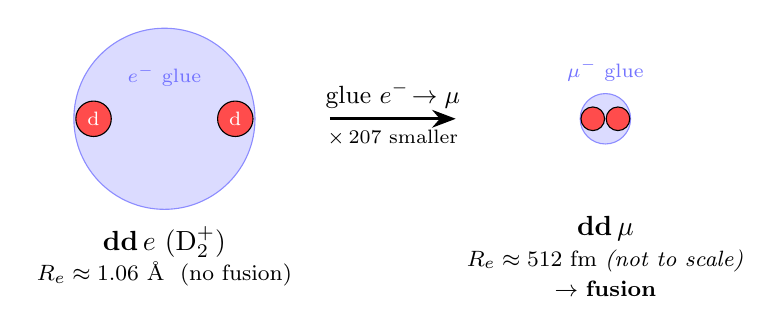
\begin{tikzpicture}[scale=1.0,
  deut/.style={circle,draw,fill=red!70,text=white,minimum size=4.5mm,inner sep=0pt,font=\scriptsize},
  glue/.style={circle,draw,fill=blue!14,draw=blue!45},
  ar/.style={-{Stealth[length=3mm]},very thick}]

 % electron-bound molecule (big)
 \draw[glue] (0,0) circle (1.15);
 \node[deut] at (-0.9,0) {d};
 \node[deut] at (0.9,0) {d};
 \node[font=\scriptsize,blue!55] at (0,0.55) {$e^-$ glue};
 \node[align=center] at (0,-1.75) {\textbf{dd$\,e$} ($\mathrm{D}_2^{+}$)\\[-1pt]\footnotesize $R_e\approx1.06$~\AA\ \ (no fusion)};

 % arrow
 \draw[ar] (2.1,0) -- (3.7,0) node[midway,above,font=\small] {glue $e^-\!\to\mu$}
   node[midway,below,font=\scriptsize] {$\times\,207$ smaller};

 % muon-bound molecule (tiny) -- drawn small, "not to scale"
 \begin{scope}[shift={(5.6,0)}]
   \draw[glue] (0,0) circle (0.32);
   \node[deut,minimum size=3mm] (dl) at (-0.16,0) {};
   \node[deut,minimum size=3mm] (dr) at (0.16,0) {};
   \node[font=\scriptsize,blue!55,above=1pt] at (0,0.32) {$\mu^-$ glue};
   \node[align=center] at (0,-1.75) {\textbf{dd$\,\mu$}\\[-1pt]\footnotesize $R_e\approx512$~fm \emph{(not to scale)}\\[-1pt]\footnotesize $\to$ \textbf{fusion}};
 \end{scope}
\end{tikzpicture}
\caption{Muon catalysis as a change of glue. The electron-bound deuteron molecular ion holds its two
deuterons about an {\aa}ngstr\"om apart and does not fuse; replacing the electron with a muon --- a
$\sim\!200\times$ smaller negative charge --- contracts the same Coulomb molecule to $\sim\!512$~fm
(drawn far larger than to scale),
close enough for the residual barrier to be tunnelled and the pair to fuse.}
\label{fig:molecules}
\end{figure}

\begin{table}[h]
\centering
\small
\setlength{\tabcolsep}{5pt}
\renewcommand{\arraystretch}{1.2}
\begin{tabular}{lccll}
\toprule
glue & scale (rel.) & $R_e$ & lifetime & fate\\
\midrule
electron $e^-$ & $1$       & $2\,a_0\approx1.06\times10^{5}$~fm & stable        & long-lived but too big: no fusion\\
muon $\mu^-$   & $1/207$   & $\approx512$~fm                    & $2.2~\mu$s    & small \emph{and} long-lived enough: fuses\\
tau $\tau^-$   & $1/3477$  & $\approx30$~fm                     & $0.29$~ps     & small enough but decays first: no catalysis\\
\bottomrule
\end{tabular}
\caption{The deuteron molecular ion with the three charged-lepton glues. Length scales as the glue scale
$c$ (depth as $1/c$), per Eq.~\eqref{eq:scaling}; only the glue's size differs. The muon is the sweet
spot --- the only lepton at once small-scale enough to compress the pair and long-lived enough to act;
the electron is too big and the tau, though smaller still, decays $\sim\!10^{7}$ times too fast to be
captured. (Conventionally the scale is written
$c=\hbar^2/2m$, so the muon's smaller scale is labelled by its larger mass.)}
\label{tab:glue}
\end{table}

\section{From separation to fusion}

Compression buys fusion because the tunnelling probability through the residual internuclear Coulomb
barrier is exponentially sensitive to the separation at which the two deuterons are held. Schematically
the barrier-penetration factor is $\exp(-G)$ with a Gamow exponent $G\propto\sqrt{R_e}$ for a Coulomb
barrier down to nuclear contact, so contracting $R_e$ by $\sim\!200$ raises the penetrability by a huge
factor and turns an immeasurably slow process into a fast one. Quantitatively the muon-bound
$\mathrm{dd}\mu$ molecule fuses at a rate of order $10^{9}~\mathrm{s^{-1}}$, and the analogous
$\mathrm{dt}\mu$ (deuteron--triton) molecule --- the practical choice, and the one on which reactor-scale
$\mu$CF studies concentrate --- at $\sim\!10^{12}~\mathrm{s^{-1}}$~\cite{Breunlich}. Either rate is
enormous compared with the inverse muon lifetime, $1/\tau_\mu\approx4.5\times10^{5}~\mathrm{s^{-1}}$
($\tau_\mu=2.2~\mu$s), so once the muon-bound molecule forms, fusion is essentially certain. The
electron-bound molecule, by contrast, has $R_e$ larger by $\sim\!200$ and a penetrability smaller by
astronomical factors: it never fuses. The whole difference is the glue's scale acting through
Eq.~\eqref{eq:scaling}.

The internal structure of each fusing deuteron, and the fusion itself, are treated in RealNucleus in the
same Coulomb terms: a deuteron is $2p+1e$, and $\mathrm{d}+\mathrm{d}\to{}^4\mathrm{He}$ is computed
directly as the merging of two such dual-confined units into the alpha~\cite{Johnson-RealNucleus}. The
muon in $\mu$CF plays no part in that final step; it is the \emph{delivery} mechanism --- the heavy glue
that brings the two deuterons into contact --- and it is released when they fuse.

\section{The catalytic cycle and its limits}

The muon is a catalyst in the exact chemical sense. Liberated when the pair fuses, it is free to bind
another two nuclei into a new tiny molecule and drive another fusion, and so on, once per cycle of
duration set by the molecular-formation and fusion rates. Two facts bound how many times this can
happen, and they are the reason $\mu$CF, though real and demonstrated, is not a power source.

\emph{The muon decays.} With a lifetime $\tau_\mu=2.2~\mu$s the muon can complete only a finite number
of cycles; at the achievable cycling rates this is of order $10^2$--$10^3$ fusions per muon before the
muon is gone.

\emph{The muon sticks.} With small but nonzero probability the muon, instead of being released, remains
bound to the newly formed $\alpha$ (a muonic helium ion) and is lost to catalysis. For the
deuteron--triton cycle this $\alpha$-sticking probability is $\omega_s\approx0.4$--$0.6\%$, which caps
the number of catalysed fusions at roughly $1/\omega_s\approx150$--$250$ regardless of the muon
lifetime.

At $\sim\!150$ fusions of $17.6$~MeV each, one muon yields $\sim\!2.6$~GeV, while producing a muon costs
of order several GeV once accelerator and pion-production inefficiencies are included. The cycle
therefore lands near, but below, break-even. Nothing in the RealNucleus reading changes this
accounting: the framework clarifies the \emph{mechanism} --- fusion as a molecule with smaller glue ---
but the Coulomb barrier, the muon lifetime, and the sticking loss are all still there. There is no free
lunch, only a clear picture of the trade.

\section{What the RealNucleus reading adds}

The value of the picture is conceptual economy. Muon catalysis is often presented as a special
low-energy nuclear phenomenon; here it is nothing but the deuteron molecular ion of
Eq.~\eqref{eq:energy} with one number changed, the glue scale $c$. The same size$\,\propto\,c$
law that shrinks the atom to the nucleus in the unified Coulomb picture~\cite{Johnson-Unified} shrinks
the electron molecule to the muon molecule, and the muon molecule fuses for the same reason a nucleus
is small: it lives at a smaller scale. Two consequences follow that are worth
developing. First, the framework makes the \emph{glue} the controllable variable, and the three charged
leptons span a clean \emph{size--lifetime trade-off} (Table~\ref{tab:glue}). Smaller scale means tighter
compression: the tau, at $\sim\!1/3477$ the electron scale, would hold the pair at $\sim\!30$~fm,
tighter even than the muon's $\sim\!512$~fm. But smaller-scale leptons are shorter-lived --- the tau
survives only $\sim\!0.29$~ps, some $10^{7}$ times less than the muon, far too briefly to be slowed,
captured, and formed into a molecule before it decays. The electron, at the other end, is stable but
too large to bring the deuterons near. The \emph{muon alone} is both small enough to compress the pair
and long-lived enough ($2.2~\mu$s) to act --- which is exactly why it, and not its lighter or heavier
siblings, is the practical catalyst. Second, the framework places ordinary \emph{electron screening}
enhancement of fusion --- a measured effect in which bound or plasma electrons modestly lower the
barrier --- on the same axis as muon catalysis: both are the negative glue drawing the nuclei together,
differing only in $c$. A quantitative RealQM treatment of that continuum, from electron screening
through to full muon catalysis, is the natural next step.

\section{Conclusion}

Muon-catalyzed fusion is the deuteron molecular ion with smaller glue. In the RealQM/RealNucleus
framework a molecular ion is two nuclei bound by a shared negative charge whose \emph{scale} $c$ sets the
bond size, so replacing the electron by the muon --- a negative charge some $200\times$ smaller ---
contracts the same Coulomb molecule from $\sim\!1$~{\AA} to $\sim\!512$~fm --- close enough that the
residual barrier tunnels and the deuterons fuse. The catalytic cycle and its ceilings (muon lifetime,
$\alpha$-sticking) follow without embellishment, and keep it below break-even. What the picture offers
is unity: the same size$\,\propto\,c$ law that separates atom from nucleus separates the inert
electron molecule from the fusing muon molecule, and puts electron screening and muon catalysis on one
continuous scale. The operative variable is size throughout; that one conventionally writes
$c=\hbar^2/2m$ only labels the scale by a mass, which belongs, with gravitation, elsewhere.

\section*{Code and simulations}
\sloppy
The deuteron molecular-ion curve, the $1/m$ rescaling to the muon case, and the underlying
$\mathrm{d}+\mathrm{d}\to{}^4\mathrm{He}$ fusion are computed with an open-source WebGPU RealQM solver,
runnable from the interactive gallery~\cite{Gallery} at
\url{https://claes542.github.io/RealMolecule/gallery.html}; see the deuteron (\path{nucleus_2h.html}),
the D\,$+$\,D fusion sweep (\path{nucleus_DD_fusion_Rsweep.html}), the muon-catalyzed fusion cycle
(\path{muon_catalyzed_fusion.html}), and the electron-versus-muon glue comparison
(\path{muon_vs_deuteron.html}).
\fussy

\section*{Acknowledgements}
The physical argument and model are the author's; the numerical implementation was developed and run
with AI assistance (Claude, Anthropic).

\begin{thebibliography}{9}
\bibitem{Frank} F.~C.~Frank, \emph{Hypothetical Alternative Energy Sources for the ``Second Meson''
Events}, Nature \textbf{160}, 525 (1947).
\bibitem{Sakharov} A.~D.~Sakharov, \emph{Passive mesons} (report, 1948); reprinted in \emph{Collected
Scientific Works} (1982).
\bibitem{Alvarez} L.~W.~Alvarez \emph{et al.}, \emph{Catalysis of Nuclear Reactions by $\mu$ Mesons},
Phys. Rev. \textbf{105}, 1127 (1957).
\bibitem{Jackson} J.~D.~Jackson, \emph{Catalysis of Nuclear Reactions between Hydrogen Isotopes by
$\mu^-$ Mesons}, Phys. Rev. \textbf{106}, 330 (1957).
\bibitem{Jones} S.~E.~Jones \emph{et al.}, \emph{Observation of Unexpected Density Effects in
Muon-Catalyzed $d$--$t$ Fusion}, Phys. Rev. Lett. \textbf{51}, 1757 (1983).
\bibitem{Breunlich} W.~H.~Breunlich, P.~Kammel, J.~S.~Cohen, M.~Leon, \emph{Muon-Catalyzed Fusion},
Ann. Rev. Nucl. Part. Sci. \textbf{39}, 311 (1989).
\bibitem{Johnson-RealNucleus} C.~Johnson, \emph{RealNucleus: Nuclear Binding as Dual Coulomb
Confinement, without a Strong or Weak Force} (companion paper).
\bibitem{Johnson-Unified} C.~Johnson, \emph{Unified Coulomb Theory for Atom and Nuclear Physics}
(companion paper).
\bibitem{Johnson-RealQM} C.~Johnson, \emph{RealQM: A Real Quantum Mechanics},
\url{https://realqm.blogspot.com}.
\bibitem{Gallery} C.~Johnson, \emph{RealMolecule / RealQM interactive simulation gallery},
\url{https://claes542.github.io/RealMolecule/gallery.html}; source
\url{https://github.com/Claes542/RealMolecule}.
\end{thebibliography}

\end{document}
